\chapter{Evaluación}
\label{sec:estudiorend}

En este capítulo describiremos las aplicaciones descritas para evaluar la integración \textit{COMPSs+OmpSs-2}, los entornos donde haremos la evaluación y los resultados de esta.  

\section{Aplicaciones}
\subsection{K-Means}

\textit{K-Means} es un algoritmo utilizado para hacer \textit{clustering} sobre un grupo de datos, es decir, agrupar los datos en \textit{clusters}. Cada dato pertenece al \textit{cluster} cuyo centro está en la distancia mínima, si no fuera así pertenecería a otro \textit{cluster}. Se inicializan \textit{clusters} con centros escogidos de manera aleatoria y se comparan las distancias a todos los \textit{clusters} y se determina a cual pertenece cada dato (siempre al centro más cercano), una vez hecho esto se vuelve a calcular el centro de cada \textit{cluster}, todo este proceso conforma una iteración de \textit{K-Means}, habitualmente se itera hasta que converge, esto es que la distancia entre los centros asignados en dos iteraciones consecutivas de cada \textit{cluster} es cercana a 0.

\begin{figure}[h]
	\centering 
	\caption{Grafo de dependencias entre tareas de K-Means.}
	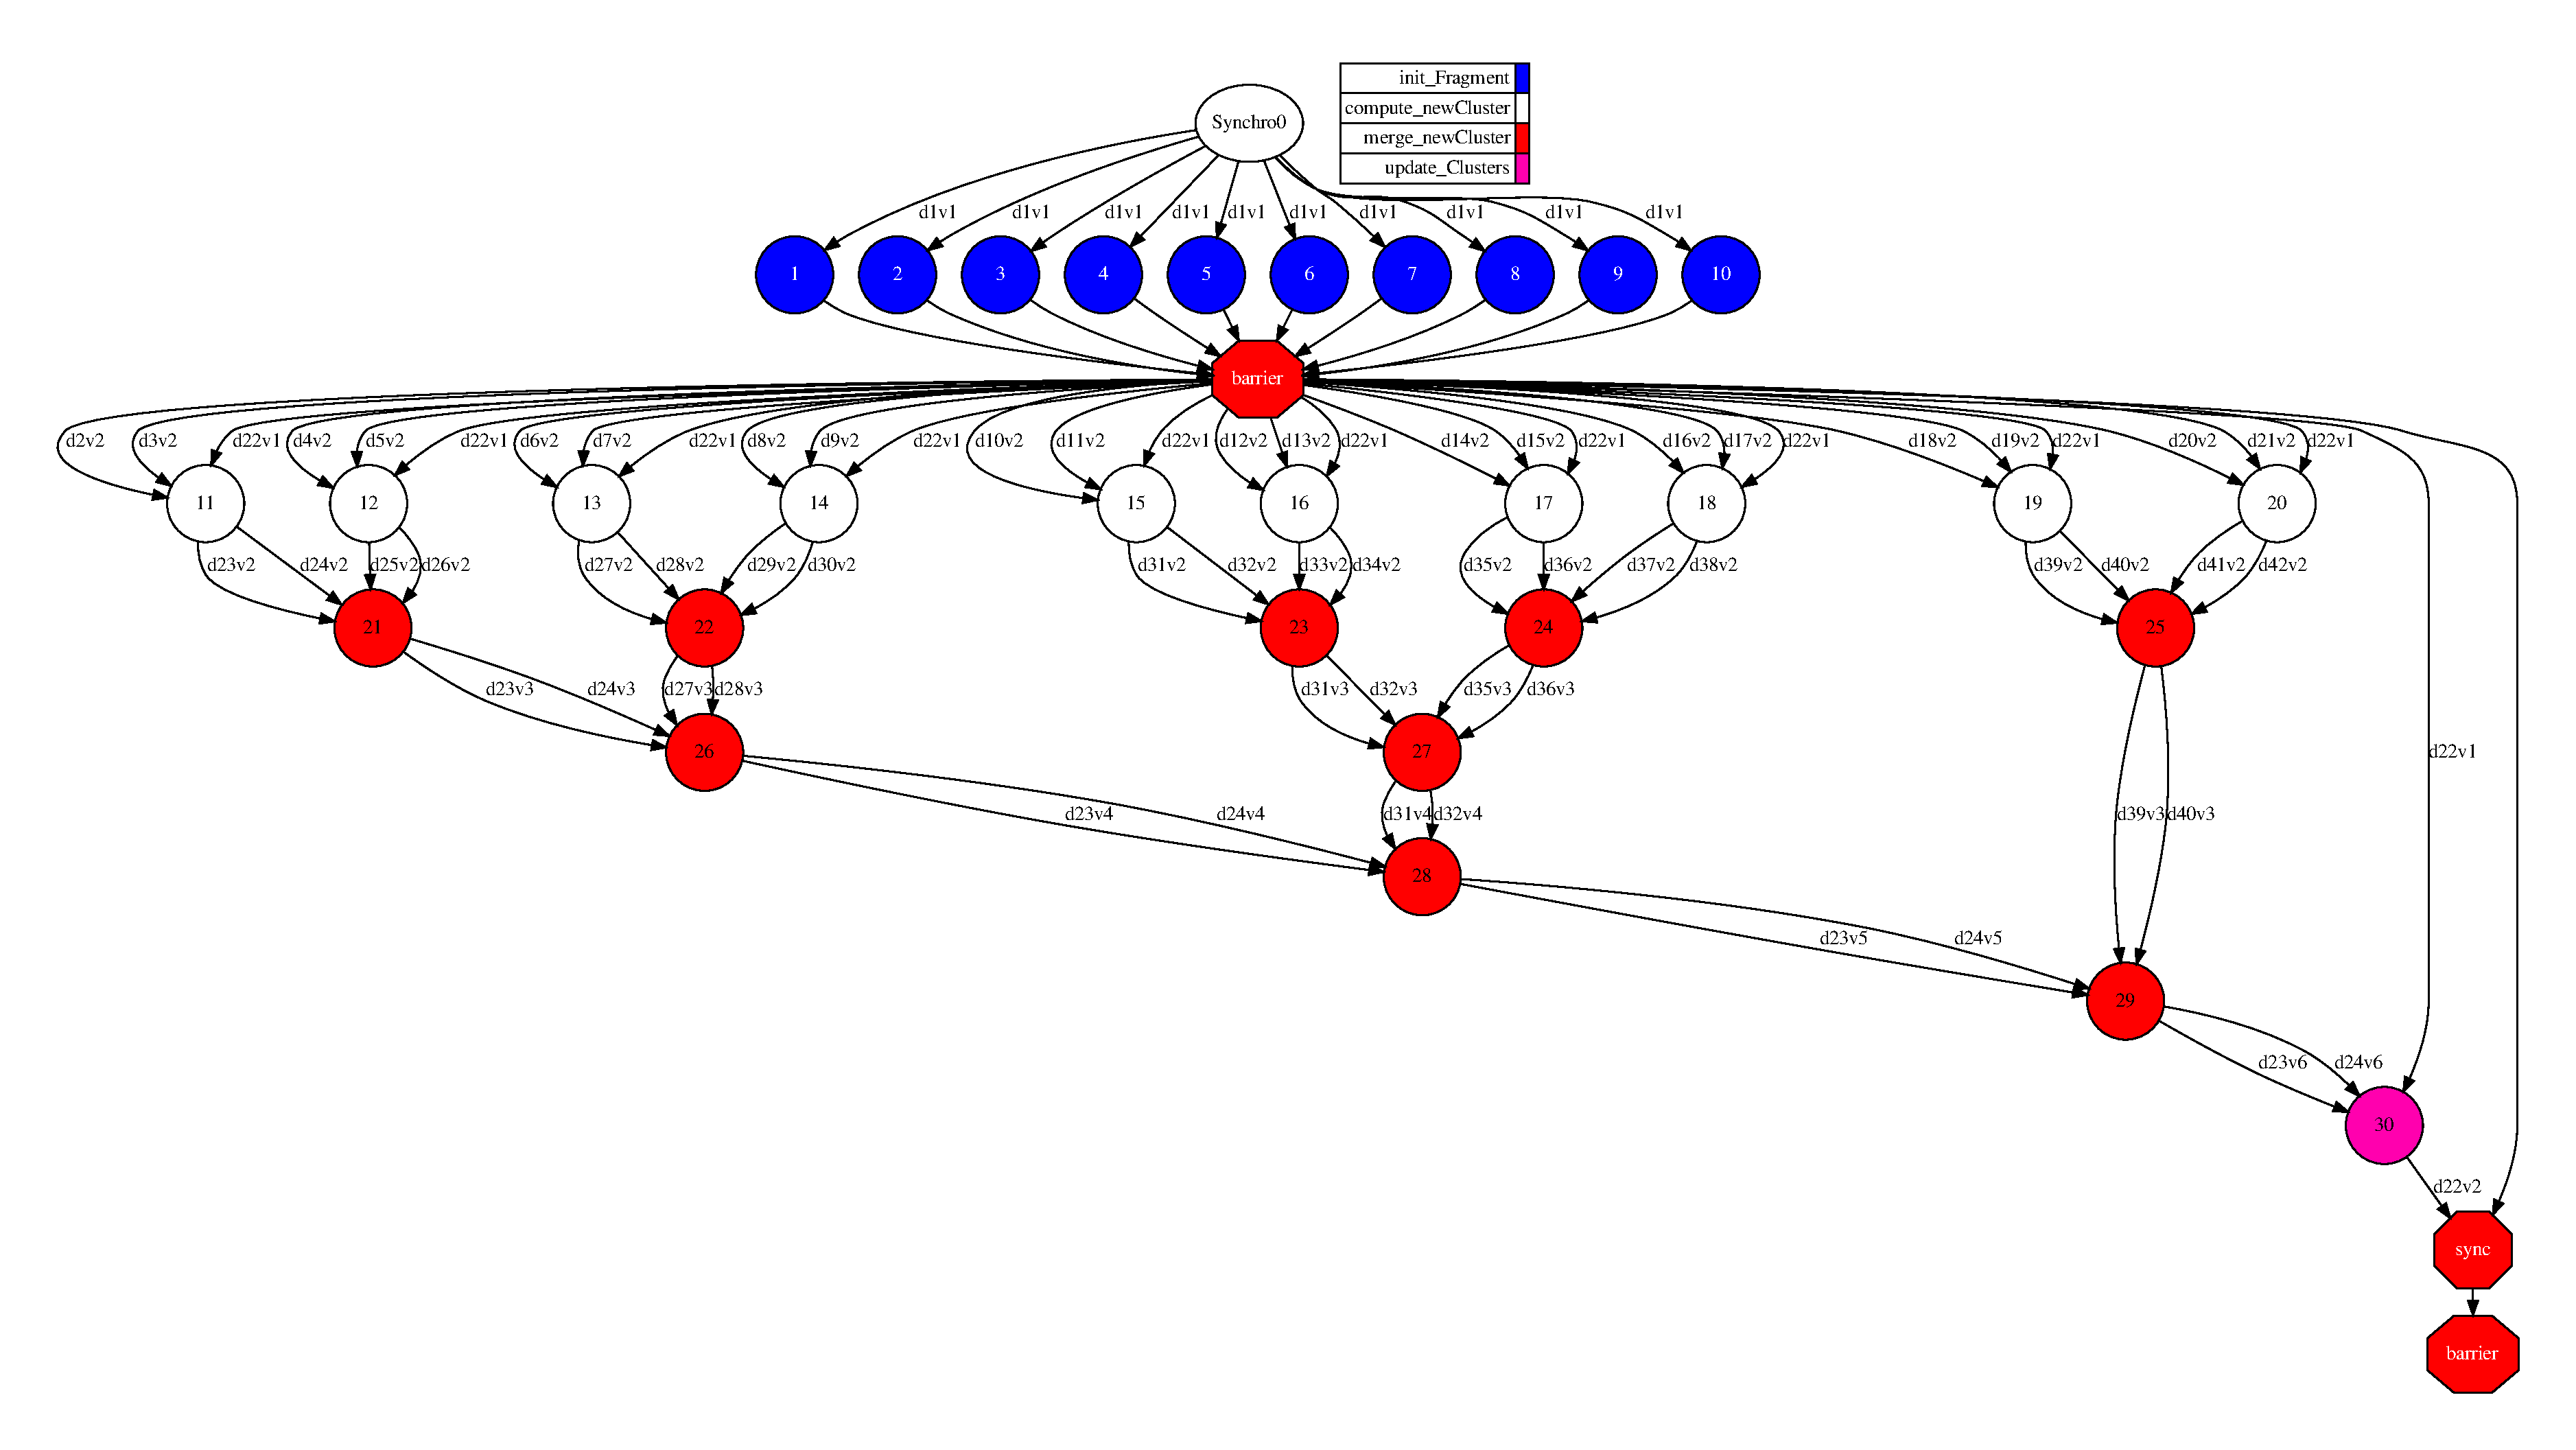
\includegraphics[scale=0.3]{grafo_kmeans.pdf}
	\label{fig:grafokmeans}
\end{figure}

Tal y como hemos desarrollado la aplicación tiene 4 tareas, que son \textit{init\_Fragment}, \textit{compute\_newCluster} (tiene una implementación en CPU y otra en GPU), \textit{merge\_newCluster}, \textit{update\_Clusters}. La imagen \ref{fig:grafokmeans} muestra un grafo de dependencias de una ejecución de \textit{K-Means} donde el número de \textit{clusters} a formar es 50 y se efectúan dos iteración. Para no sobrecargar este apartado se incluye en el apéndice \ref{sec:codigokmeans} la interfaz y el programa principal de la aplicación.

\subsection{Cholesky}

\textit{Cholesky} es un método de descomposición aplicable cuando la matriz es simétrica definida positiva, entonces esta puede ser descompuesta como el producto de una matriz triangular inferior y su traspuesta. El método \textit{Cholesky} se utiliza para resolver sistemas de ecuaciones lineales, es similar a la descomposición \textit{LU} y es el doble de eficiente.
\par\bigskip
La aplicación ha sido desarrollada utilizando una librería para operaciones de algebra lineal programada en \textit{C} con \textit{OmpSs} y \textit{OmpSs-2}, esta librería es \textit{LASs}\footnote{https://pm.bsc.es/mathlibs/lass} (\textit{Linear Algebra routines on OmpSs}). Las funciones que implementa \textit{LASs} serán utilizadas como tareas a nivel de \textit{COMPSs} y después una vez ejecutadas harán uso de \textit{OmpSs-2}, por lo que realmente desarrollar una aplicación utilizando una librería externa es muy sencillo.
\par\bigskip
Tiene 5 tareas, \textit{generate\_block}, \textit{ddss\_dpotrf}, \textit{ddss\_dtrsm}, \textit{ddss\_dgemm}, \textit{ddss\_dsyrk}, \textit{generate\_block} se utiliza para generar los bloques de manera distribuida (así el \textit{master} no tiene reservar memoria para toda la matriz, que podría ser muy grande), las otras 4 tareas son operaciones de algebra lineal que utilizadas de la forma correcta aplicarán el método de descomposición de \textit{Cholesky}.
En el apéndice \ref{sec:codigocholesky} se encuentra la interfaz y el programa principal de la aplicación. 

\begin{figure}[h]
	\centering 
	\caption{Grafo de dependencias entre tareas de Cholesky.}
	\includegraphics[scale=0.12]{grafo_cholesky.pdf}
	\label{fig:grafocholesky}
\end{figure}

La imagen \ref{fig:grafocholesky} muestra un grafo de dependencias de la aplicación \textit{Cholesky} con una matriz de 64 bloques con 4096x4096 elementos cada uno. 

\section{Entornos para el estudio}

Para la realización del estudio del rendimiento se han utilizado dos máquinas que el \textit{Barcelona Supercomputing Center} pone a nuestra disposición, que son \textit{CTE-Power} y \textit{MareNostrum4}.

\subsection{CTE-Power}
\label{sec:power}

\textit{CTE-Power} es un \textit{cluster} basado en la tecnología de procesadores \textit{IBM} \textit{Power9}. Tiene 2 nodos de \textit{login}, son los nodos desde donde operan los usuarios y 52 nodos de cómputo. 
\par\smallskip
Cada nodo tiene los siguientes componentes:
\par\smallskip
\begin{itemize}
	\item 2 x \textit{IBM Power9 8335-GTH} @ 2.4GHz (3.0GHz en modo turbo), cada procesador con 20 cores cada uno con 4 \textit{threads}.
	\item 512GB de memoria organizada en 16 \textit{dimms} de 32GB @ 2666MHz.
	\item 4 x \textit{NVIDIA} V100 con 16GB \textit{HBM2}.
	\item 2 x SSD que proporcionan 1.9TB de almacenaje local.
	\item 2 x \textit{NVM Express} 3.2TB.
	\item Interfaz de red \textit{Mellanox}.
	\item Sistema de ficheros GPFS a través de fibra a 10GBit.
\end{itemize}

Nosotros utilizaremos tan sólo 10 nodos, por lo que tendremos a nuestra disposición en la mayor ejecución 1600 CPUs y 40 GPUs \textit{NVIDIA V100}. 

\subsection{MareNostrum4}
\label{sec:mare}

\textit{MareNostrum4} es un supercomputador basado en la tecnología de procesadores \textit{Intel Xeon Platinum} de la generación \textit{Skylake}. Tiene 5 nodos de \textit{login} y 3.456 nodos de cómputo.
\par\smallskip
Cada nodo tiene los siguientes componentes:
\par\smallskip
\begin{itemize}
	\item 2 x \textit{Intel Xeon Platinum 8160 @ 2.10GHz} con 24 cores.
	\item Hay nodos con distintos tipos de memoria:
		\subitem 1,88 GB/core de memoria. %organizada en 12 \textit{dimms} de 8GB @ 2667MHz.
		\subitem 7,93 GB/core de memoria.
	\item Un SSD que proporciona 200 GB de almacenaje local.
	\item 100 Gbit/s \textit{Intel Omni-Path HFI Silicon 100 Series PCI-E adapter}.
	\item 10 Gbit \textit{Ethernet}.
\end{itemize}

Igual que con \textit{CTE-Power} tan sólo utilizaremos 10  nodos, por lo tanto tendremos en la mayor ejecución 480 CPUs.

\section{K-Means}

La evaluación con \textit{K-Means} ha consistido en hacer un test de \textit{strong scaling}, que consiste en ejecutar la aplicación con un tamaño de problema fijo y aumentar el número de recursos de cómputo, y otro de \textit{weak scaling} donde aumentaremos de manera proporcional el tamaño del problema y los recursos de cómputo. En el apartado \ref{sec:power} describimos la máquina que utilizamos en estos test, haremos uso de todas las \textit{CPUs} y \textit{GPUs} de cada nodo.

\subsection{Strong scaling}

La imagen \ref{fig:sc-time} muestra una gráfica que tiene en el eje vertical el tiempo y en el horizontal el número de nodos. El tamaño del problema que se ha utilizado es de 400 fragmentos de 50 dimensiones y 200000 puntos cada uno, el número de \textit{clusters} a formar es 50 y se efectúan 5 iteraciones. Se han tomado 10 muestras de cada ejecución, la línea azul muestra la media de las muestras para el mismo número de nodos, la de color naranja muestra el tiempo ideal que debería tardar según el número de nodos. En cada punto de la línea azul se muestra la diferencia entre el máximo valor y el mínimo que se han tomado en las muestras.

\begin{figure}[H]
	\centering 
	\caption{Tiempo de ejecución al aumentar el número de recursos.}
	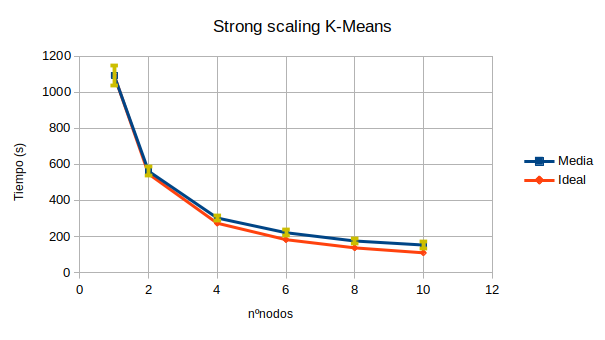
\includegraphics[scale=0.8]{estudio/KMeans/sc/kmeans-sc-time.png}
	\label{fig:sc-time}
\end{figure}

Es bueno que la línea azul sea lo más parecida a la línea naranja, eso nos indicaría que la aplicación escala perfectamente, ya que cada vez que aumentamos los recursos el tiempo de ejecución se reduciría proporcionalmente. La imagen \ref{fig:sc-speedup} muestra la misma información que \ref{fig:sc-time} dispuesta en forma de ganancia, se puede ver que se comporta bien hasta que en los 4 nodos empieza a dejar de acercarse al ideal.

\begin{figure}[H]
	\centering 
	\caption{Ganancia al aumentar el número de recursos.}
	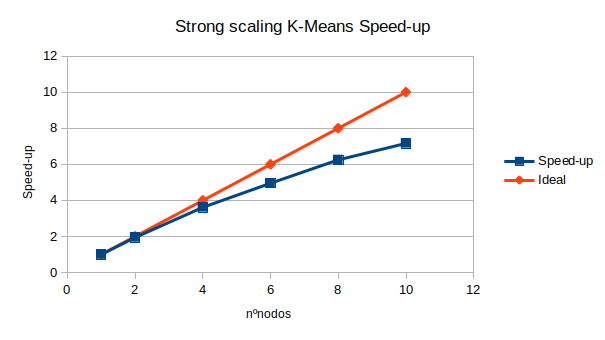
\includegraphics[scale=0.8]{estudio/KMeans/sc/kmeans-sc-speedup.png}
	\label{fig:sc-speedup}
\end{figure}
 
Esta disminución de la ganancia cobra sentido cuando en el grafo de la aplicación \ref{fig:grafokmeans} vemos que en la fase de computar los \textit{clusters} nuevos (tareas de color blanco) la aplicación es totalmente paralela pero en la fase de re-asignar los centros de los \textit{clusters} (tareas de color rojo) deja de serlo. Esta característica de la aplicación hace que nunca podamos alcanzar la ganancia ideal ya que hay tramos o fases de esta que no son completamente paralelos, aunque estemos utilizando todos los recursos que hay a nuestra disposición tenemos que esperar a ejecutar un nivel de re-asignación antes de empezar el siguiente. 

\subsection{Weak scaling}

En un test de \textit{weak scaling}, esperamos que los tiempos de ejecución sean siempre los mismos, ya que el tamaño del problema es siempre proporcional a los recursos de cómputo. Esto sería perfecto pero hay que efectuar comunicación entre nodos y gestionar todo el sistema, por lo que no podemos mantener este escenario ideal. La imagen \ref{fig:wc-effic} muestra cómo al aumentar el número de nodos la eficiencia baja del ideal (que el tiempo de ejecución sea siempre el mismo), pero se mantiene alrededor del mismo valor a partir de los 6 nodos.

\begin{figure}[H]
	\centering 
	\caption{Eficiencia al mantener proporcional el tamaño del problema y el número de recursos.}
	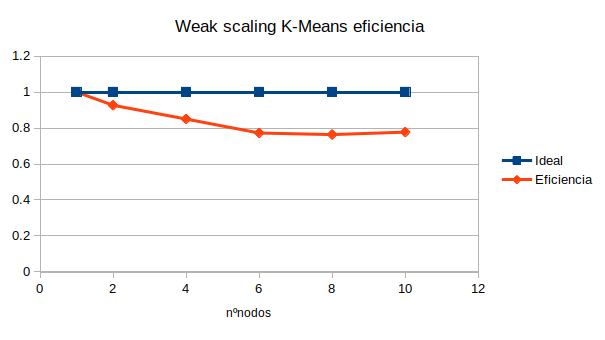
\includegraphics[scale=0.8]{estudio/KMeans/wc/kmeans-wc-efficiency.png}
	\label{fig:wc-effic}
\end{figure}

\section{Cholesky}

Para evaluar la integración con la aplicación \textit{Cholesky} hemos decidido comparar la integración \textit{COMPSs+OmpSs-2} con \textit{COMPSs} puro, en el primer test de la evaluación hemos variado el número de bloques y el tamaño de estos bloques. La evaluación con esta aplicación se lleva acabo en un nodo de \textit{MareNostrum4} que se han descrito en la sección \ref{sec:mare}.

\par\bigskip

\begin{figure}[H]
	\centering 
	\caption{Tiempo de ejecución de Cholesky con 16 bloques.}
	\includegraphics[scale=0.8]{estudio/Cholesky/cholesky-16-blocks-time.png}
	\label{fig:cholesky-16-time}
\end{figure}

La imagen \ref{fig:cholesky-16-time} muestra el tiempo de ejecución de la versión \textit{COMPSs+OmpSs-2} y \textit{COMPSs} con 16 bloques, los tamaños de bloque aparecen en el eje horizontal. A medida que se aumenta el tamaño de cada bloque la librería \textit{LASs} tiene más margen para partir los bloques y generar tareas, pero la versión \textit{COMPSs} ejecuta todo absolutamente en secuencial, haciendo que cada vez que la ganancia sea más notoria. En la imagen \ref{fig:cholesky-16-speedup} se muestra la ganancia de \textit{COMPSs+OmpSs-2} respecto la versión de \textit{COMPSs}.

\par\bigskip

\begin{figure}[H]
	\centering 
	\caption{Ganancia de Cholesky con COMPSs+OmpSs-2 respecto la versión COMPSs.}
	\includegraphics[scale=0.8]{estudio/Cholesky/cholesky-16-blocks-speedup.png}
	\label{fig:cholesky-16-speedup}
\end{figure}

A pesar de que en las imágenes \ref{fig:cholesky-16-time} y \ref{fig:cholesky-16-speedup} se muestra una diferencia grande entre la versión con y sin \textit{OmpSs-2}, esto es así por que el número de tareas que \textit{COMPSs} puede generar y están libres de dependencias y por tanto puede ejecutar a la vez no es superior o igual al número de procesadores que hay en un nodo, por este motivo no estamos aprovechando todo el nodo. En cambio en la versión con \textit{OmpSs-2} partimos los bloques y generamos tareas que los procesen, estas utilizan los procesadores que en cualquier otro caso estarían inactivos.

\par\bigskip

Tal y como hemos visto, las gráficas anteriores no eran justas para \textit{COMPSs} ya que no permitían utilizar todos los procesadores del nodo. El siguiente test pretende poner ambas versiones en un escenario justo, el número de bloques se aumenta a 64 y los tamaños de bloque se mantienen como en el anterior test.
\par\bigskip

La imagen \ref{fig:cholesky-64-time} muestra los tiempos de ejecución de ambas versiones, por el mismo motivo que antes al aumentar el tamaño de bloque las diferencias entre ambas se vuelven más notorias.

\par\bigskip

\begin{figure}[H]
	\centering 
	\caption{Tiempo de ejecución de Cholesky con 64 bloques.}
	\includegraphics[scale=0.8]{estudio/Cholesky/cholesky-64-blocks-time.png}
	\label{fig:cholesky-64-time}
\end{figure}

Es en la ganancia de la imagen \ref{fig:cholesky-64-speedup} donde se puede apreciar que la comparación es más justa que la anterior, ahora como máximo obtenemos una ganancia alrededor de 3.5, antes estaba cerca de 10. Ha sido el aumento del número de bloques lo que ha permitido que la versión de \textit{COMPSs} aproveche todo un nodo. Aún así, si vemos la imagen \ref{fig:grafocholesky} se puede ver como en la aplicación el número de tareas disminuye a medida que se acaba la aplicación, por lo que nos volvemos a encontrar en el mismo escenario anterior, en el cual no aprovechábamos todos los recursos del nodo. \textit{COMPSs+OmpSs-2} vuelve a sacar provecho de este escenario, puesto que aunque haya menos tareas de granularidad gruesa, estas generan de granularidad finas al nivel de \textit{OmpSs-2} con lo cual se puede seguir aprovechando los recursos.

\par\bigskip

\begin{figure}[H]
	\centering 
	\caption{Ganancia de Cholesky con COMPSs+OmpSs-2 respecto la versión COMPSs.}
	\includegraphics[scale=0.8]{estudio/Cholesky/cholesky-64-blocks-speedup.png}
	\label{fig:cholesky-64-speedup}
\end{figure}










